\documentclass{article}
\usepackage{amsmath}
\usepackage{amsfonts}
\usepackage{amssymb}
\usepackage{cancel}

\usepackage{graphicx}


\setlength\parindent{0pt}

\author{Pranav Tikkawar}
\title{Workshop 3}

\begin{document}
\maketitle
\begin{enumerate}
    \item $x'(t) = [x(t)]^2 $
    \begin{enumerate}
        \item - \begin{itemize}
            \item  If we consider the equation $x'(t) = [x(t)]^2 = v(x(t))$ we know that $x(t_0) = x_0  $ is a sol of $x'(t)$ if $v(x_0) =0$
            \item if $x_0 = 0$ then $v(x_0) = 0 $ meaning that $0$ is the "edge" of the interval
            \item The interval then are $(-\infty , 0)$ as well as $(0 , \infty)$ 
        \end{itemize}
        \item - \begin{itemize}
            \item We can consider this DE as a seperable DE and write it in the form of $F(x(t))x'(t) = G(t) $ we can have $F(x(t)) = \frac{1}{x^2}$ and $G(t) = 1 $
            \item We can now integrate both sides: $\int_{}^{}\frac{1}{x^2}dx = \int_{}^{}dt $
            \item As a result we get $\frac{-1}{x} = t + C $
            \item Solving for $C$ we get $C = \frac{-1-t_0x_0}{x_0} $
            \item Solving for $x(t)$ we get $x(t) = \frac{1}{-t +1/x_0 + t_0}$  
        \end{itemize}
        \item - \begin{itemize}
            \item It will take infinte time both in the past and future to reach $x=0$ as we can notice that $x(t)$ behaves similar to $-1/t$ 
            \item $\lim_{t \rightarrow \infty}x(t) = 0$ 
            \item $\lim_{t \rightarrow -\infty}x(t) = 0$
        \end{itemize}
        \item - \begin{itemize}
            \item We know that $0$ is the equilibrium state for this DE as $x_0 = 0$ solves $v(x_0) = 0$ so the other solutions for other starting $x_0$ cannot cross over $0$
            \item Since we are given that $x_0 > 0$ for our initial condition we need to see the interval of time that $x(t)$ in our previous equation where $x(t) > 0$
            \item That interval is $(-\infty, \frac{1+t_0x_0}{x_0}) $
        \end{itemize}
        \item - \begin{itemize}
            \item We can use the FTC to ensure a unique solution to this DE as we are given a initial condition that is on a continous interval ***
        \end{itemize}
        \item - \begin{enumerate}
            \item [a] Same as (a) in the previous question, $(-\infty , 0)$ as well as $(0 , \infty)$ 
            \item [b] Same as (b) $x(t) = \frac{1}{-t +1/x_0 + t_0}$
            \item [c] Same as (c) it takes infinite time both past and future
            \item [d] This is not the same, it is infact the interval where $x(t) < 0$ which is $(\frac{1+t_0x_0}{x_0}, \infty) $
            \item [e] This is the same as before
        \end{enumerate}
        \item - \begin{itemize}
            \item Because it takes infinite time to reach $x=0$ for all the intial values $x_0 \ne 0 $ then it stands to reason that $x=0$ is the unique solution for the DE
        \end{itemize}
        \item - \begin{itemize}
            \item Graph at bottom
            \item The relations between the graphs is that they are similar graphs just shifted right by 2. They also have aymptotes that are 2 units away from each other
        \end{itemize}
        \item - \begin{itemize}
            \item We can use and example to prove that the function is not well defined on that interval
            \item We can recognize that the function itself is not well defined on the interval for $x_0 = \frac{1}{t_1 - t_0} $ 
            \item If we consider $t_1 > t_0$ we can see that $x_0 $ is a positive number, but the flow transomraiton is not well defined which is what we were looking for
        \end{itemize}
        \item - \begin{itemize}
            \item For this IVP we can solve it using a guess as we can rewrite $y(t) = u(t) + x(t)$ and $y'(t) = u'(t) + x'(t) $ where we suppose $x(t) $ is a solution to the DE which we guess is $x(t) = 3t $
            \item We can expand out $y'(t) = 3 + (3t)^2 - 6ty(t) + (y(t))^2$ 
            \item Replacing $y(t) = u(t) + x(t)$ we get $u'(t) + x'(t) = 3 + (3t)^2 - 6t(u(t) + x(t)) + (u(t) + x(t))^2 $
            \item We then notice with regrouping the facting some terms cancel as $x(t)$ is a sol to the DE $u'(t) + x'(t) = 3 + (3t)^2 - 6tx(t) +(x(t))^2 - 6tu(t) + 2u(t)x(t) + (u(t))^2$
            \item Canceling $x'(t) $ and replacing $x(t) =3t $ we get $u'(t) = (u(t))^2 $
            \item From the previous question we see that $u(t) = \frac{-1}{t+C}$
            \item $y(t) = \frac{-1}{t+C} + 3t $ where $C = \frac{1}{3t_0 -y} - t_0 $
        \end{itemize}
    \end{enumerate}
    
\end{enumerate}

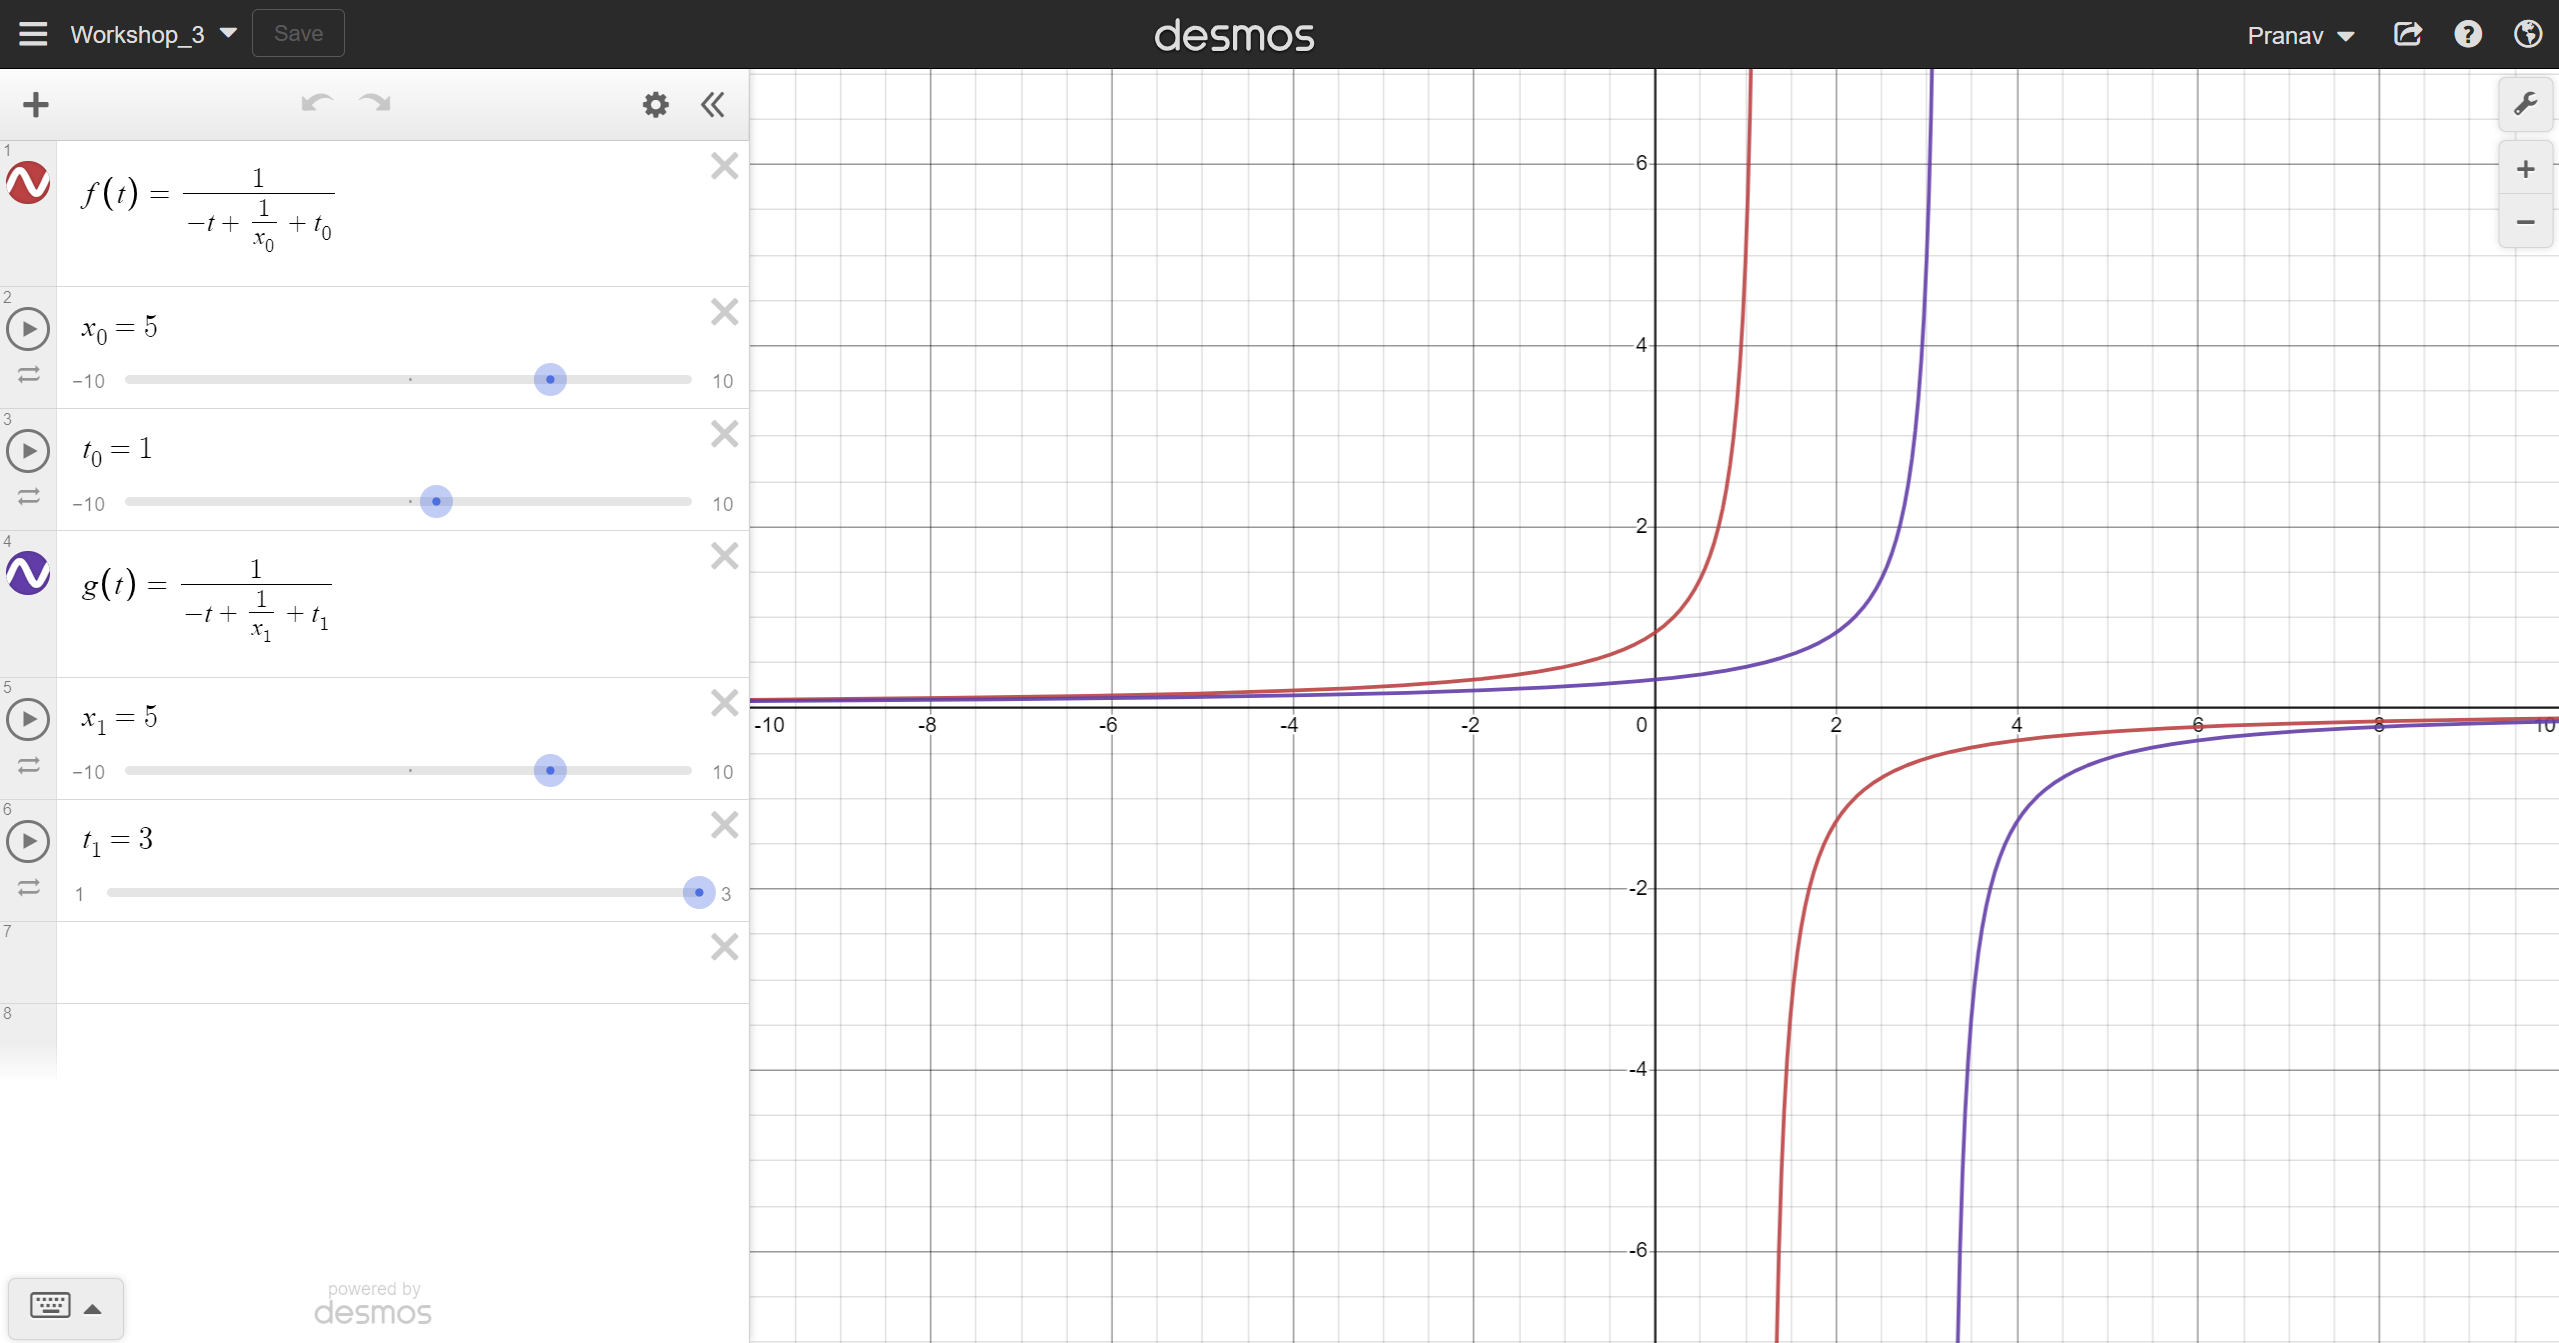
\includegraphics[scale=.2]{IVP_3.png}

\end{document}